\documentclass{elteikthesis}

\usepackage[final]{pdfpages}
\usepackage{caption}
\usepackage{hyperref}
\usepackage{xcolor}
\usepackage{biblatex}
\usepackage{subfigure}

% Document's metadata
\title{Histopathologic Cancer Detection: Identifying metastatic tissue in histopathologic slides using Deep Neural Networks} 
\date{2020}

% Author's metadata
\author{Bauer Marko}
\degree{Computer Science BSc}

% Superivsor(s)' metadata
\supervisor{Kitlei Róbert}
\affiliation{assistant lecturer, MSc} 

% University's metadata
\university{Eötvös Loránd University}
\faculty{Faculty of Informatics}
\department{Department of Programming Languages\\ and Compilers}
\city{Budapest}
\logo{elte_logo}

% Add bibliography file
\addbibresource{thesis.bib}

% The document
\begin{document}
	
% Set document language
\documentlang{english}

% Some document settings
% Contiunous counting of footnotes among chapters
\counterwithout{footnote}{chapter}

% Hide page numbering of ToC
\newcounter{conpageno}
\let\oldtableofcontents\tableofcontents
\renewcommand{\tableofcontents}{
	\pagenumbering{gobble}
	\oldtableofcontents
	\cleardoublepage
	\setcounter{conpageno}{\value{page}}
	\pagenumbering{arabic}
	\setcounter{page}{\value{conpageno}}
}


% Title page
\maketitle

% Thesis topic declaration
%\setboolean{@twoside}{false}
%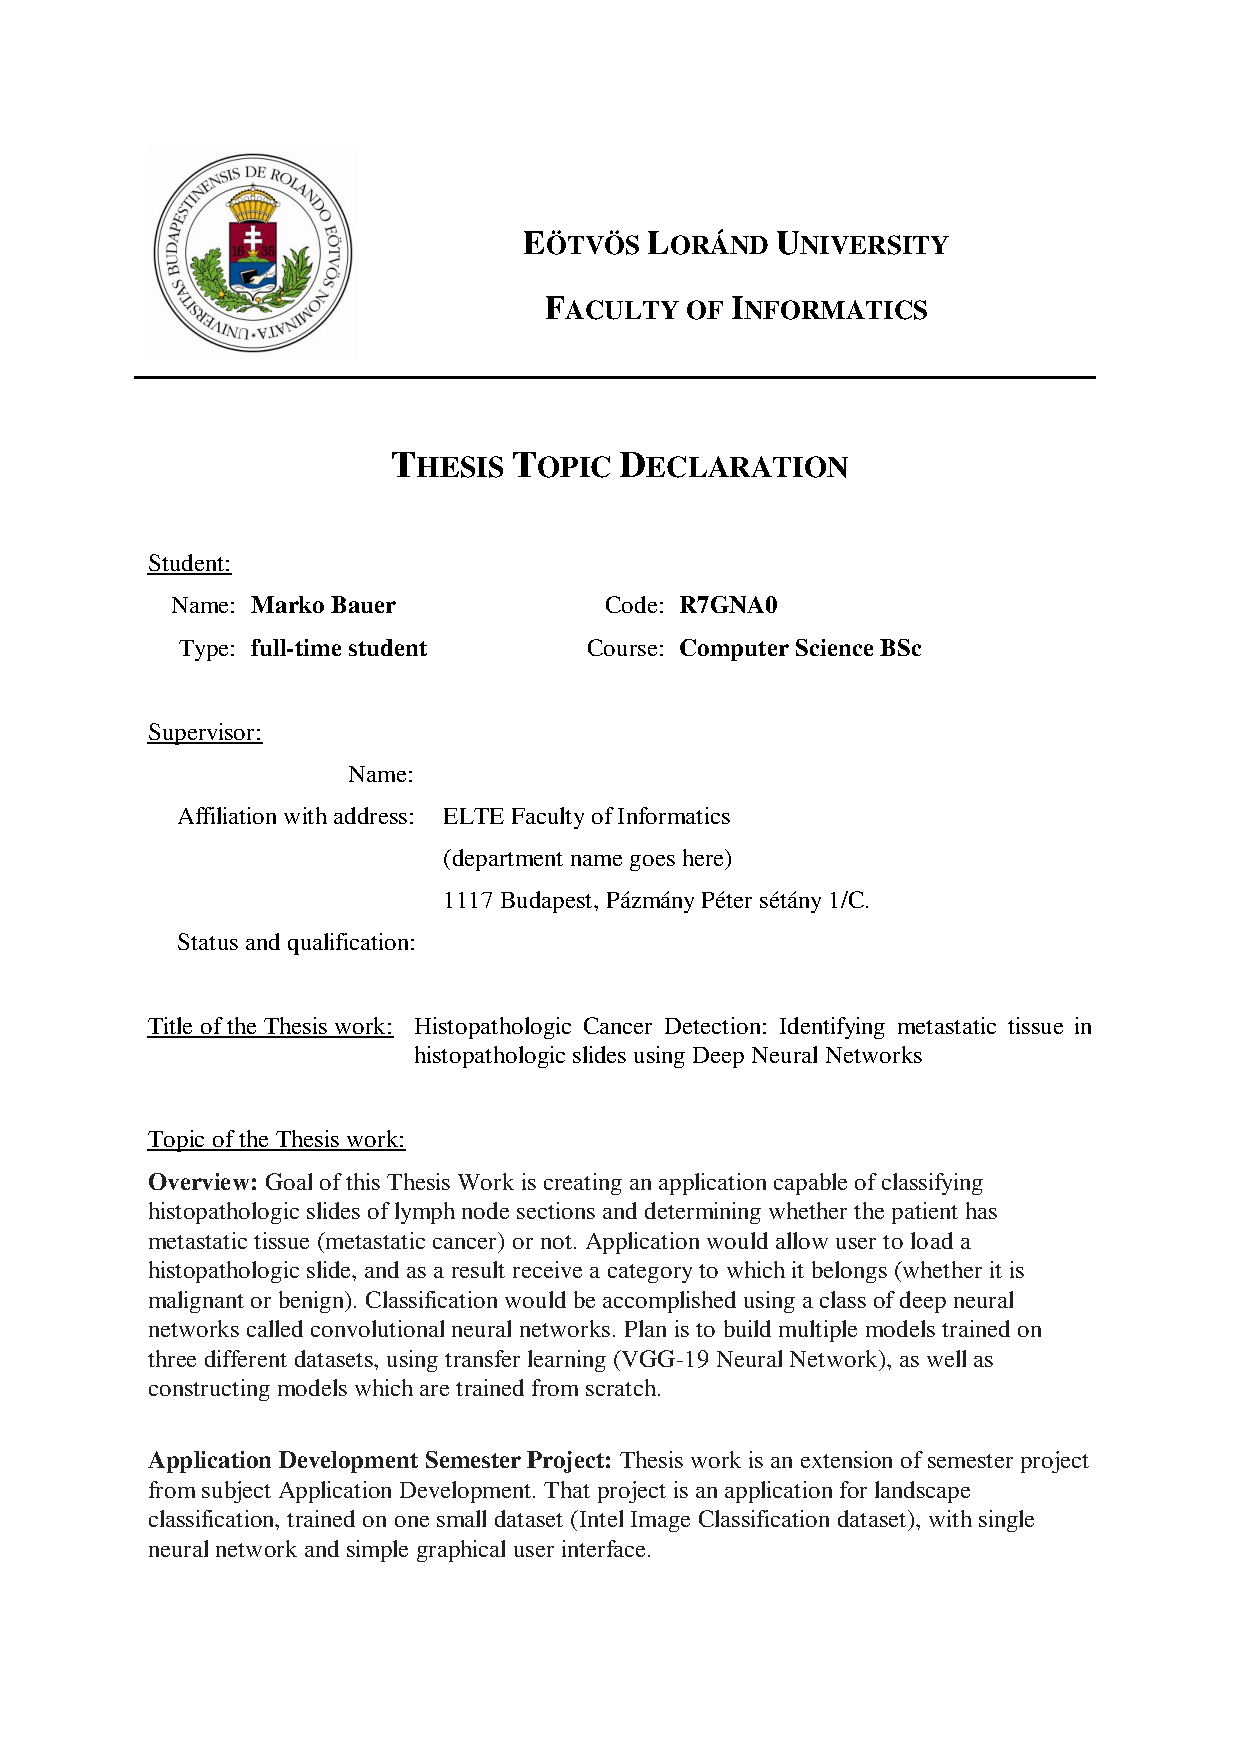
\includepdf[pages=-]{topic_declaration.pdf}
%\includepdf[pages=-]{topic_declaration_2.pdf}

% Table of contents (mandatory)
\tableofcontents
\cleardoublepage

% Main content
\chapter{Introduction}
\label{ch:intro}

Over the past decade deep learning has been reaching unimaginable heights, possibly starting another industrial revolution \cite{ml_revolution}. Numerous problems were solved with extraordinary accuracies, surpassing previous solutions, as well as human performance. Self-driving cars \cite{bojarski2016end} and automated transportation \cite{nguyen2018deep}, digital personal assistants \cite{polyakov2018investigation}, fraud detection \cite{perols2011financial}, natural language processing \cite{young2018recent} are just some of the tasks whose solutions use deep learning algorithms. But arguably the biggest impact was made in the field of computer vision \cite{voulodimos2018deep}, with image classification \cite{rawat2017deep}, object detection  and segmentation \cite{zhao2019object}, image colorization \cite{zhang2016colorful}, reconstruction \cite{wang2018image}, super-resolution \cite{dong2014learning} and synthesis \cite{reed2016generative}, and as a result, the entire healthcare industry is on a verge of a major transformation. Deep learning algorithms could be used in various ways, such as analyzing electronic health records \cite{rajkomar2018scalable}, detecting heart problems \cite{poplin2018prediction}, diagnosing cancer \cite{fakoor2013using}, planning, navigating and performing surgery \cite{shvets2018automatic}.

\section{Medical Image Analysis}

Majority of the data present in medicine (over 90\% of it) belongs to the imaging data, and it is natural to assume that deep learning could have huge impact in the future of medicine. Computed tomography (CT), magnetic resonance imaging (MRI) and X-rays are just some of the medical imaging techniques which produce data that can be used in deep learning algorithms. In this paper I will focus on analysis of histopathology slides, microscopic images of tissue obtained during biopsy.

\section{Histopathologic Cancer Detection}
Histopathologic cancer detection refers to the problem of detecting cancerous tumors in pathologic scans of lymph nodes, organs of the lymphatic system (widely present throughout the body), which act as filters for foreign particles and cancer cells. This task is clinically-relevant, as pathologists analyze a great number of histopathologic slides on a daily basis, which is time-consuming and tedious task prone to misinterpretation. Hence a lucrative solution would reduce their workload, speed up the process, and improve the prediction accuracy. In this paper, I propose a deep learning algorithm to solve this task.

\section{Datasets}
Digital pathology is field in medical imaging, where whole-slide scanners are used to digitize glass slides containing tissue at high resolution, in order to be viewed, managed, shared and analyzed on a computer. The advance of digital pathology has led to the high availability of digital images, which has in turn led to creation of datasets on which deep learning methods can be applied. In this paper, I will work with two such datasets, BreakHis and NCT-CRC-HE-100K.

\subsection{BreakHis Dataset}

The Breast Cancer Histopathological Image Classification \cite{breakhis_article} (BreakHis) is a dataset constructed in collaboration with Pathological Anatomy and Cytopathology Laboratory (Parana, Brazil) which contains 9.109 images of breast tumor tissue. It is collected from 82 patients, using different magnifying factors (40x, 100x, 200x, and 400x), and contains 2.480  benign and 5.429 malignant samples (700x460 pixels). Dataset is divided into two main groups, benign tumors (do not invade nearby tissue or spread to other parts of the body) and malignant tumors (can invade nearby tissues, made of cancer cells). Based on the way cells look under the microscope, there are eight subtypes of tumors: adenosis, fibroadenoma, phyllodes tumors and tubular adenona for benign tumors, and carcinoma, lobular carcinoma, mucinous carcinoma and papillary carcinoma for malignant tumors (\textcolor{red}{\autoref{fig:breakhis}}).

\captionsetup[figure]{font=scriptsize,labelfont=scriptsize}

\begin{figure}[h]
	\centering
	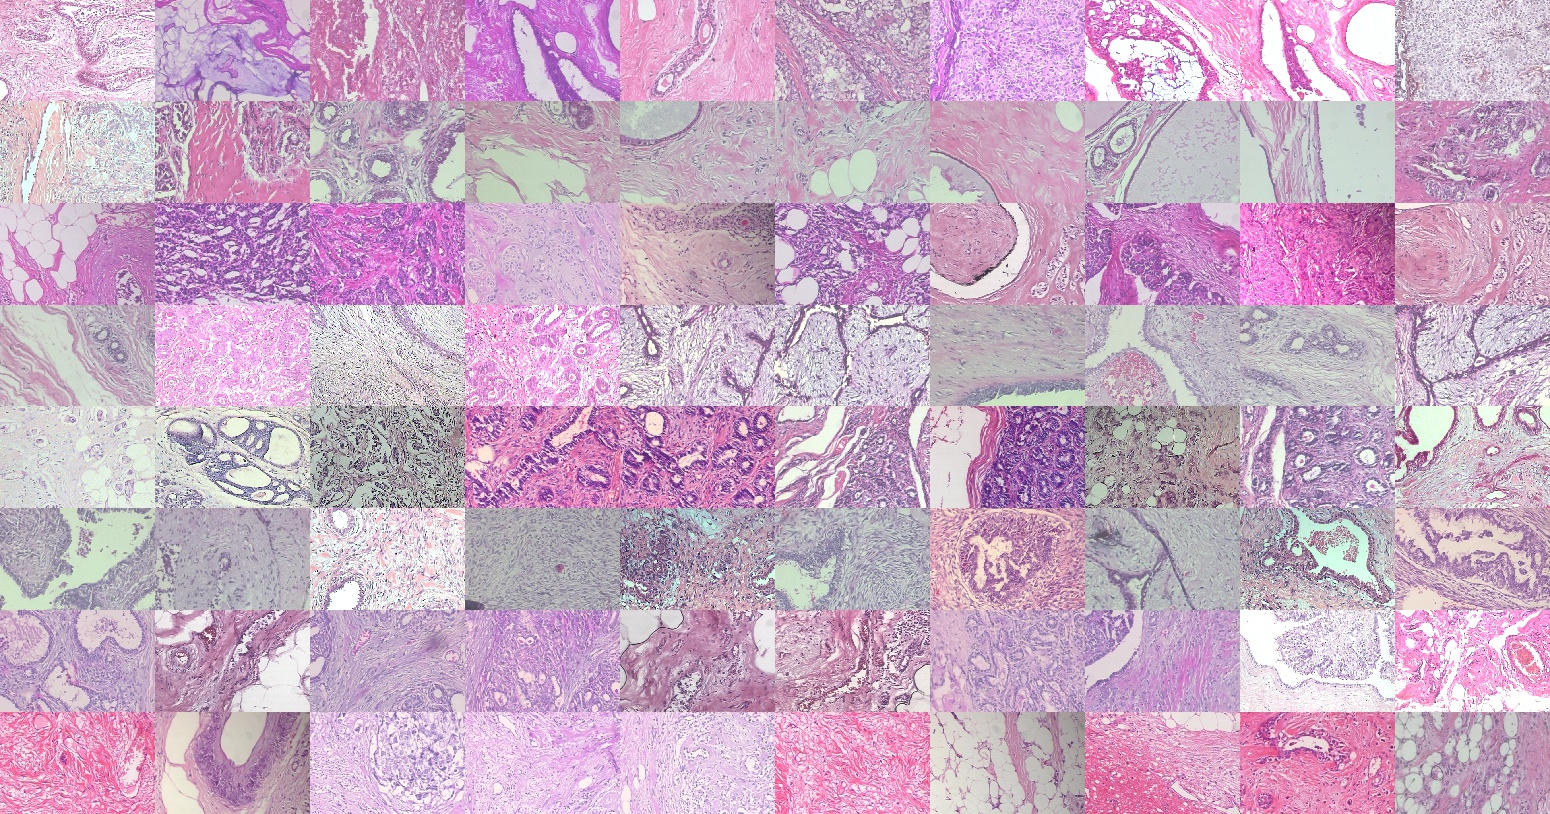
\includegraphics[scale=0.32]{break_his_dataset.jpg}
	\caption{BreakHis dataset tumor classes: adenosis, ductal carcinoma, fibroadenoma, lobular carcinoma, mucinous carcinoma, papillary carcinoma, phyllodes tumor, tubular adenoma}
	\label{fig:breakhis}
\end{figure}

\subsection{NCT-CRC-HE-100K Dataset}

The NCT-CRC-HE-100K \cite{kather_jakob_nikolas_2018_1214456} is a dataset constructed in collaboration with National Center for Tumor diseases (Heidelberg, Germany) which contains 100.000 images of colorectal tumor tissue. It is collected from 86 patients, using 100x magnifying factor (224x224 pixels). Based on the way cells look under the microscope, there are nine subtypes of tissue: adipose, background, debris, lymphocytes, mucus, smooth muscle, normal colon mucosa, cancer-associated stroma and colorectal adenocarcinoma epithelium (\textcolor{red}{\autoref{fig:nctcrche100k}}).

\begin{figure}[h]
	\centering
	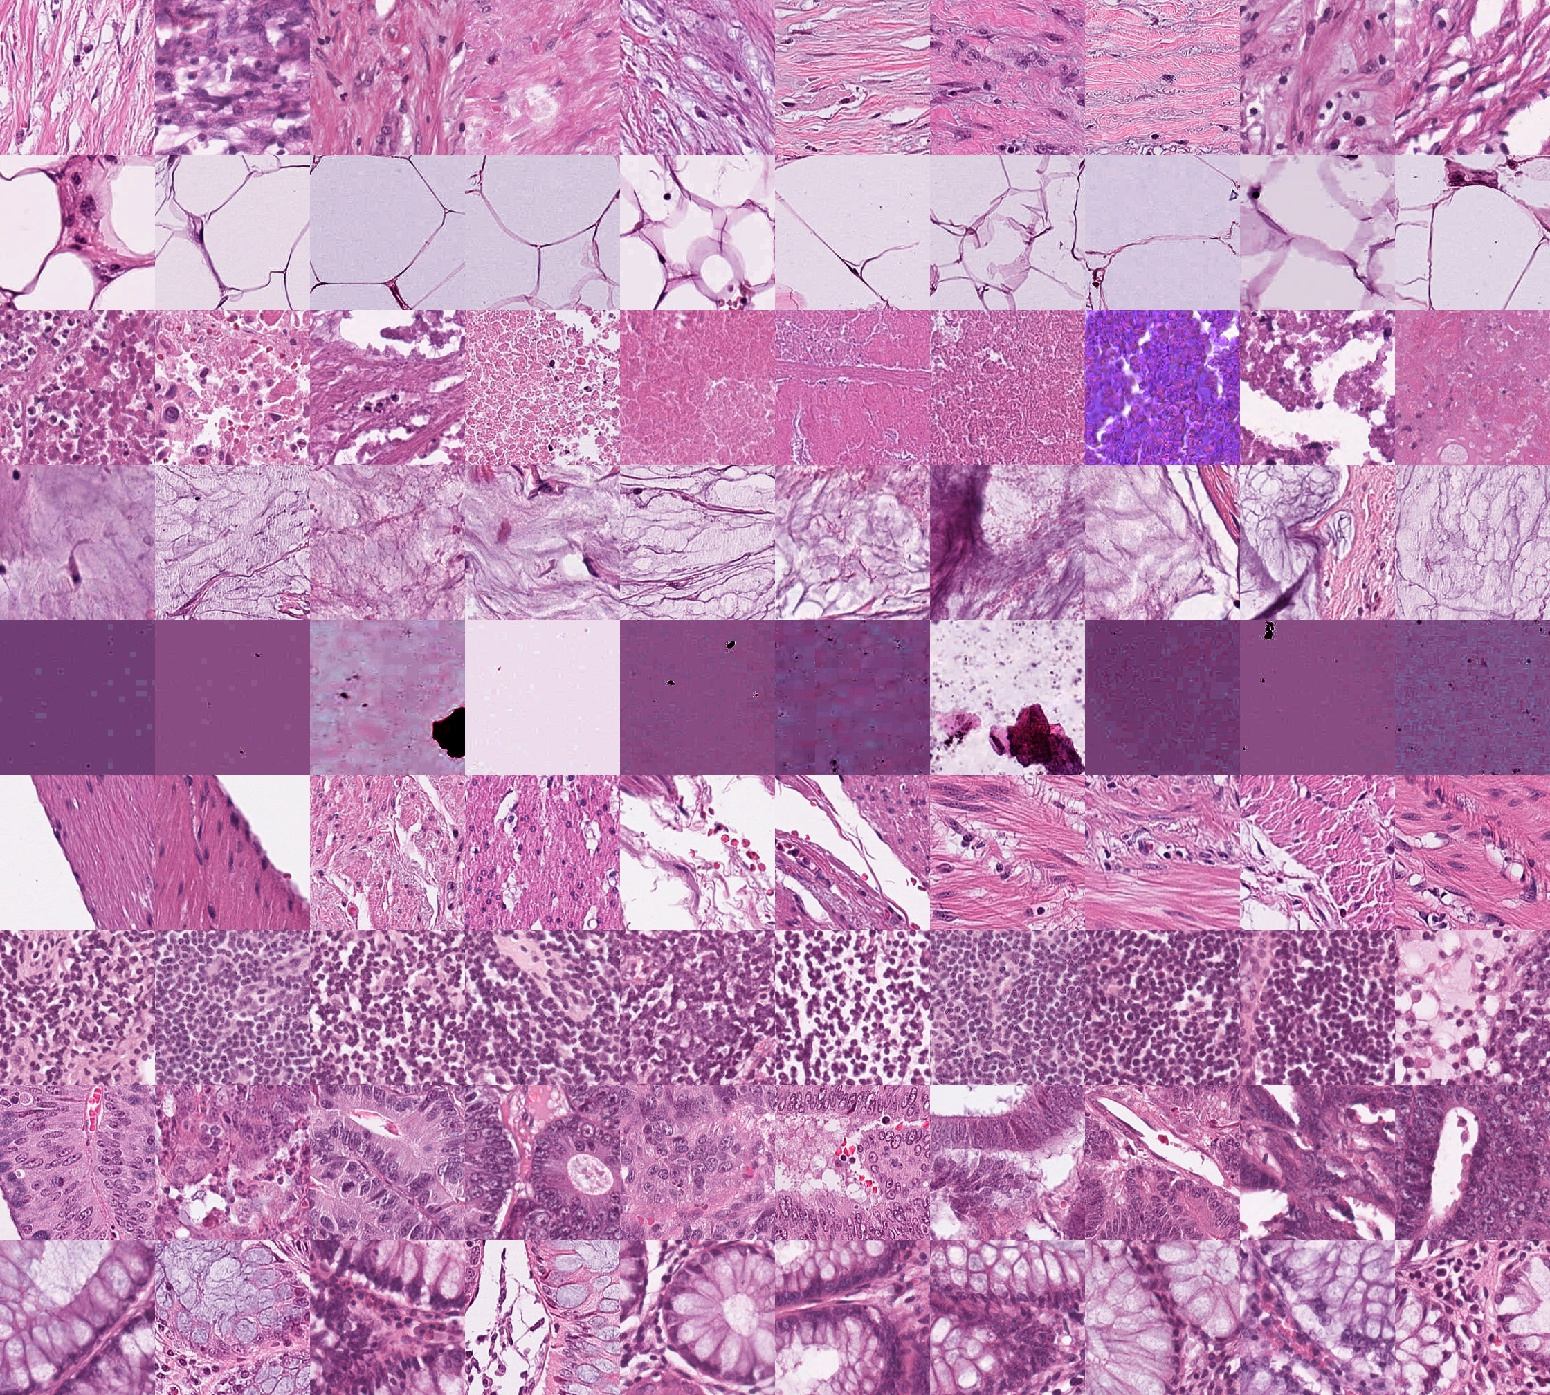
\includegraphics[scale=0.22]{nct_crc_he_100k_dataset.jpg}
	\caption{NCT-CRC-HE-100K dataset tissue classes: adipose tissue, background, debris, lymphocytes, mucus, smooth muscle, normal colon mucosa, cancer-associated stroma, colorectal adenocarcinoma epithelium}
	\label{fig:nctcrche100k}
\end{figure}

\section{Approach}

I have divided the creation of the program for histopathologic cancer detection in four major parts:
\begin{enumerate}
	\itemsep0em
	\item Assembling dataset structure (required for input to convolutional neural network), image preprocessing (loading, removing noise, normalization, whitening) and data augmentation (expanding size of dataset by applying a series of random transformations to each image)
	\item Building the convolutional neural networks (class of deep neural networks applied to analyzing images), and training them on data
	\item Improving prediction accuracy of networks (solving underfitting and overfitting problems) with hyperparameter tuning (choosing optimal parameters for learning algorithm) and changes to network architecture
	\item Creating graphical user interface for the program, which allows user to load histopathologic slide and select network which has be applied on it, and to get as output category to which that slide belongs, with additional possibility to visualize network representations (heatmaps of class activations, filters of convolutional layers and intermediate activations)
\end{enumerate}


\cleardoublepage

\chapter{User Documentation}
\label{ch:user}

There are three main ways of using Histopathologic Cancer Detection program:
\begin{enumerate}
	\itemsep 0em
	\item Predicting tissue and cancer subtype of breast and colorectal tissue, i.e. predicting whether patient has breast or colorectal cancer or not
	\item Visualizing what Convolutional Neural Network (CNN) learns, i.e. visualizing how network transforms input image, and which parts of input image lead to predicting tissue and cancer subtype
	\item Adding new datasets and networks in order to increase the scope of the program, and predict even more tissue and cancer subtypes
\end{enumerate}
Before using the program, certain system requirements need to be satisfied.

\section{System Requirements}
\label{sysreq}

In order to run Histopathologic Cancer Detection, Python 3.5+ is required on one of the following operating systems: Windows 7 or later (64bit), macOS 10.12.6 (Sierra) or later (64bit), Ubuntu 16.04 or later (64bit) or Raspbian 9.0 or later. Moreover, considering computer needs to be powerful enough to perform large number of tensor operations and handle the computing power necessary, CPU Intel Core i5 6th generation processor or higher (or an AMD equivalent processor) and 8+GB of RAM are required.

\subsection{General Software Requirements}

In order to use the program to predict tissue and cancer subtype, and to visualize what CNNs learn, following Python dependencies are required: 
\begin{itemize}
	\itemsep 0em
	\item \texttt{H5py} - interface to the HDF5 binary data format, which can store huge amounts of numerical data, and easily manipulate that data from \texttt{NumPy} (used to save and load network weights)
	\item \texttt{Keras}, \texttt{Keras-Applications}, \texttt{Keras-Preprocessing}, \texttt{TensorFlow} - neural networks APIs, which can build and deploy machine learning applications (used to build and train neural networks)
	\item \texttt{Matplotlib}, \texttt{seaborn} - data visualization libraries (used for visualization of datasets, neural networks and tissue and cancer subtype predictions)
	\item \texttt{NumPy} - library which provides support for large, multi-dimensional arrays
	\item \texttt{OpenCV-Python}, \texttt{Pillow}, \texttt{scikit-image} - image processing libraries (used to load, process and save images)
	\item \texttt{pandas} - data analysis and manipulation library (used for loading datasets)
	\item \texttt{PyQt5} - python binding of cross-platform GUI toolkit Qt, which contains substantial set of GUI widgets (used for implementing GUI part of the program)
	\item \texttt{scikit-learn} - machine learning library for predictive data analysis (used for its metrics in order to assess network performance)
\end{itemize}

\subsection{Additional Software Requirements}

In order to replicate results of already existing networks, or to expand scope of the program by adding new datasets and training new networks, NVIDIA GPU card with CUDA Compute Capability 3.5 or higher is required, along with the following:
\begin{itemize}
	\itemsep 0em
	\item NVIDIA CUDA toolkit - provides a development environment for creating high performance GPU-accelerated applications
	\item NVIDIA CUDA Deep Neural Network Library (cuDNN) - GPU-accelerated library of primitives for deep neural networks, which provides highly tuned implementations for standard routines
	\item \texttt{TensorFlow-GPU} - GPU-enabled version of \texttt{TensorFlow} library
\end{itemize}
Training convolutional neural networks requires large amount of computations, and in order to decrease training time, networks are trained on GPU (it is not feasible on CPU, as GPU training is multiple times faster).

\section{Running the Program}

After running the program, new window appears (\textcolor{red}{\autoref{fig:startup}}).

\begin{figure}[h]
	\centering
	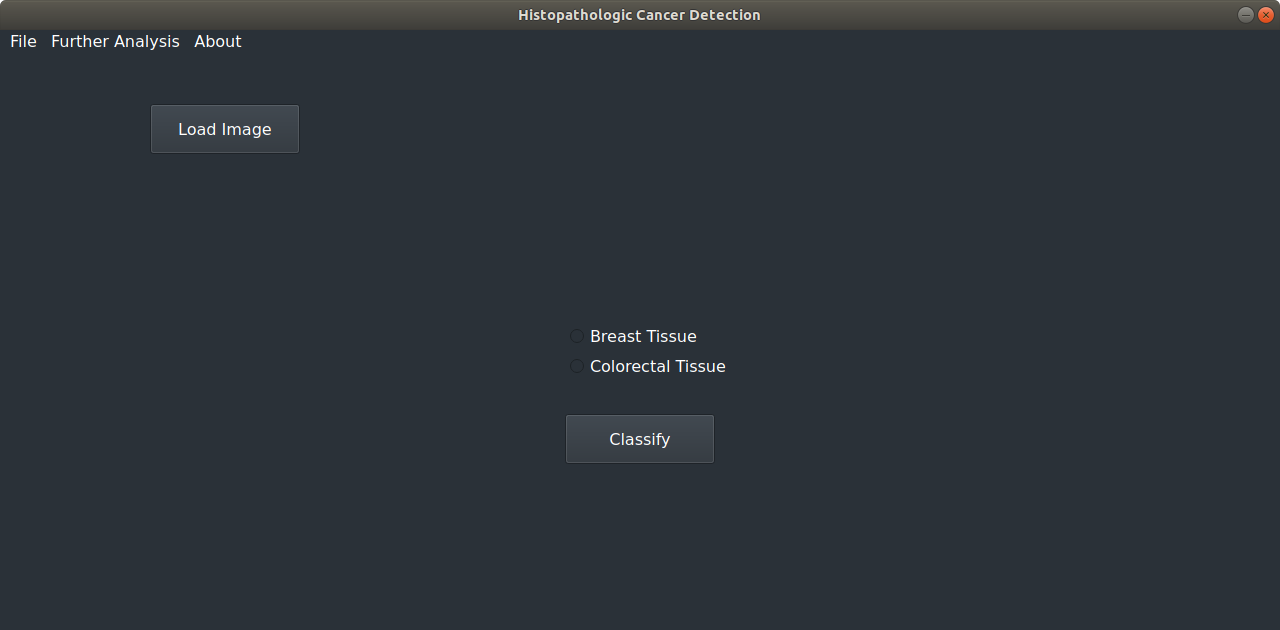
\includegraphics[scale=0.3]{startup_window.png}
	\caption{Main window of Histopathologic Cancer Detction program}
	\label{fig:startup}
\end{figure}

From here, it is possible to:
\begin{enumerate}
	\itemsep 0em
	\item Inspect datasets (\textcolor{red}{\hyperref[inspdata]{Section 2.3}}) and networks (\textcolor{red}{\hyperref[inspnets]{Section 2.4}})
	\item Load histopathologic slide of breast or colorectal tissue and predict the tissue and cancer subtype (\textcolor{red}{\hyperref[basicuse]{Section 2.5}})
	\item Further visualize network representations by analyzing heatmaps of class activations, filters of convolutional layers and intermediate \\ activations (\textcolor{red}{\hyperref[advuse]{Section 2.6}})
\end{enumerate}
\clearpage

\section{Inspecting Datasets}
\label{inspdata}

In order to find basic information about datasets, which include sample images from dataset, tissue and cancer subtypes, as well as number of images per category, go to \emph{About $\rightarrow$ About\;Datasets} and choose dataset (\textcolor{red}{\autoref{fig:inspectdataset}}). In current implementation there are two datasets available: BreakHis and NCT-CRC-HE-100K.

\begin{figure}[h]
	\centering
	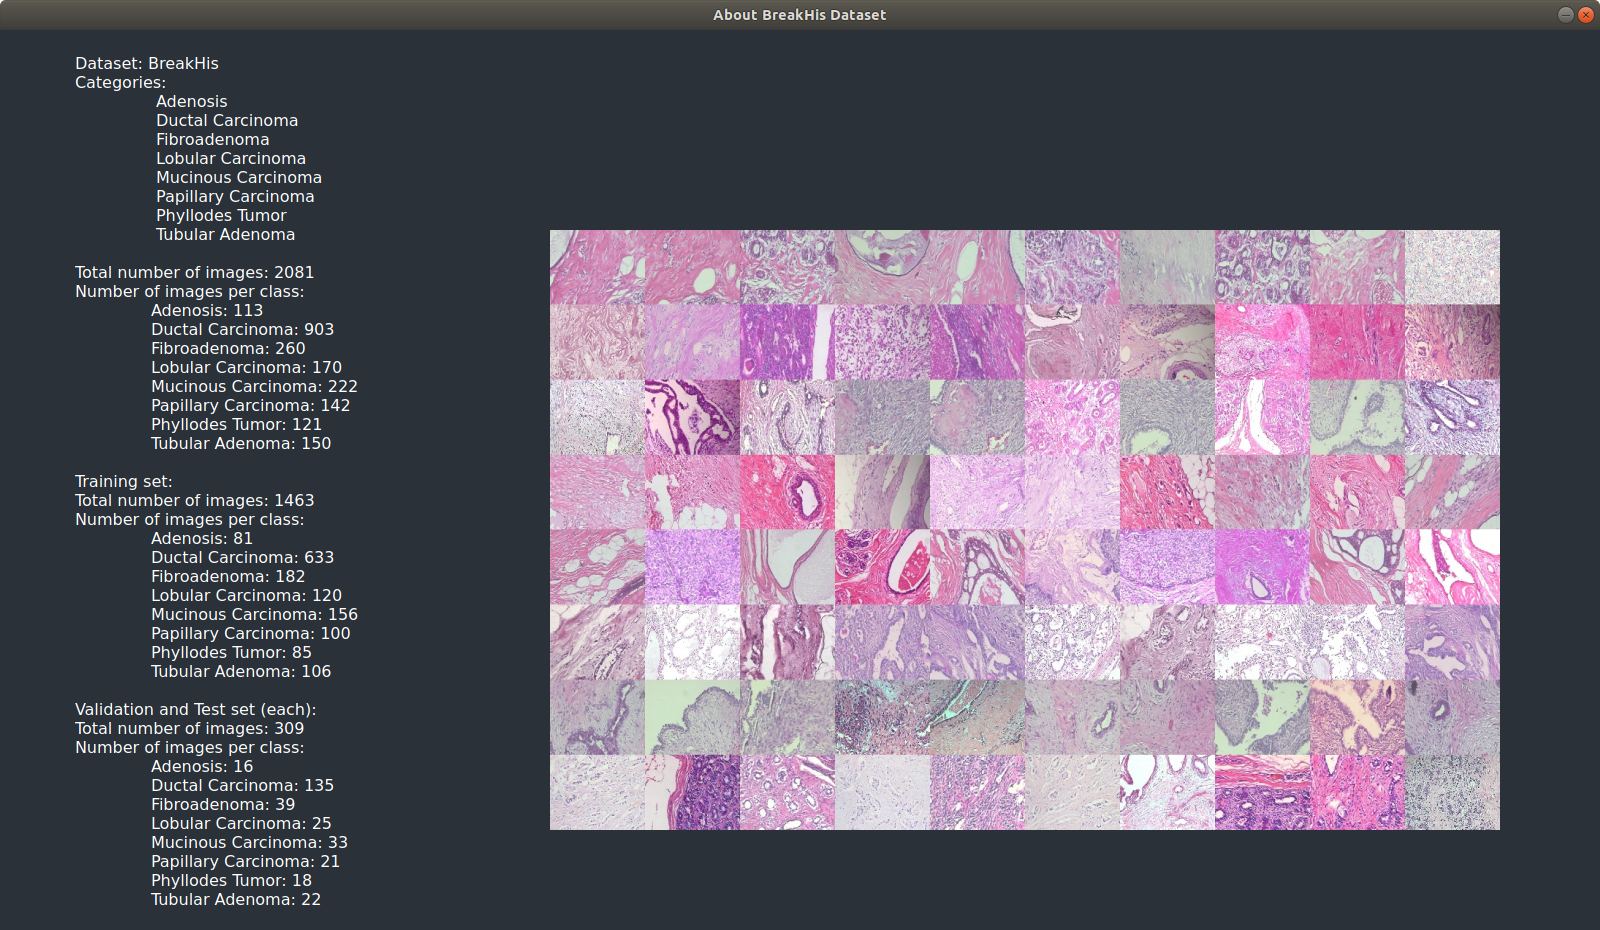
\includegraphics[scale=0.25]{inspect_dataset.png}
	\caption{BreakHis Dataset basic information}
	\label{fig:inspectdataset}
\end{figure}

\section{Inspecting Networks}
\label{inspnets}

In order to find basic information about networks, which include network architecture and network performance on training, validation and test datasets (accuracy, loss and confusion matrix), go to \emph{About $\rightarrow$ About\;Models} and choose network (\textcolor{red}{\autoref{fig:inspectmodel}}). In current implementation there are two networks available: CNNSimple and VGG19Simple.
\clearpage

\begin{figure}[h]
	\centering
	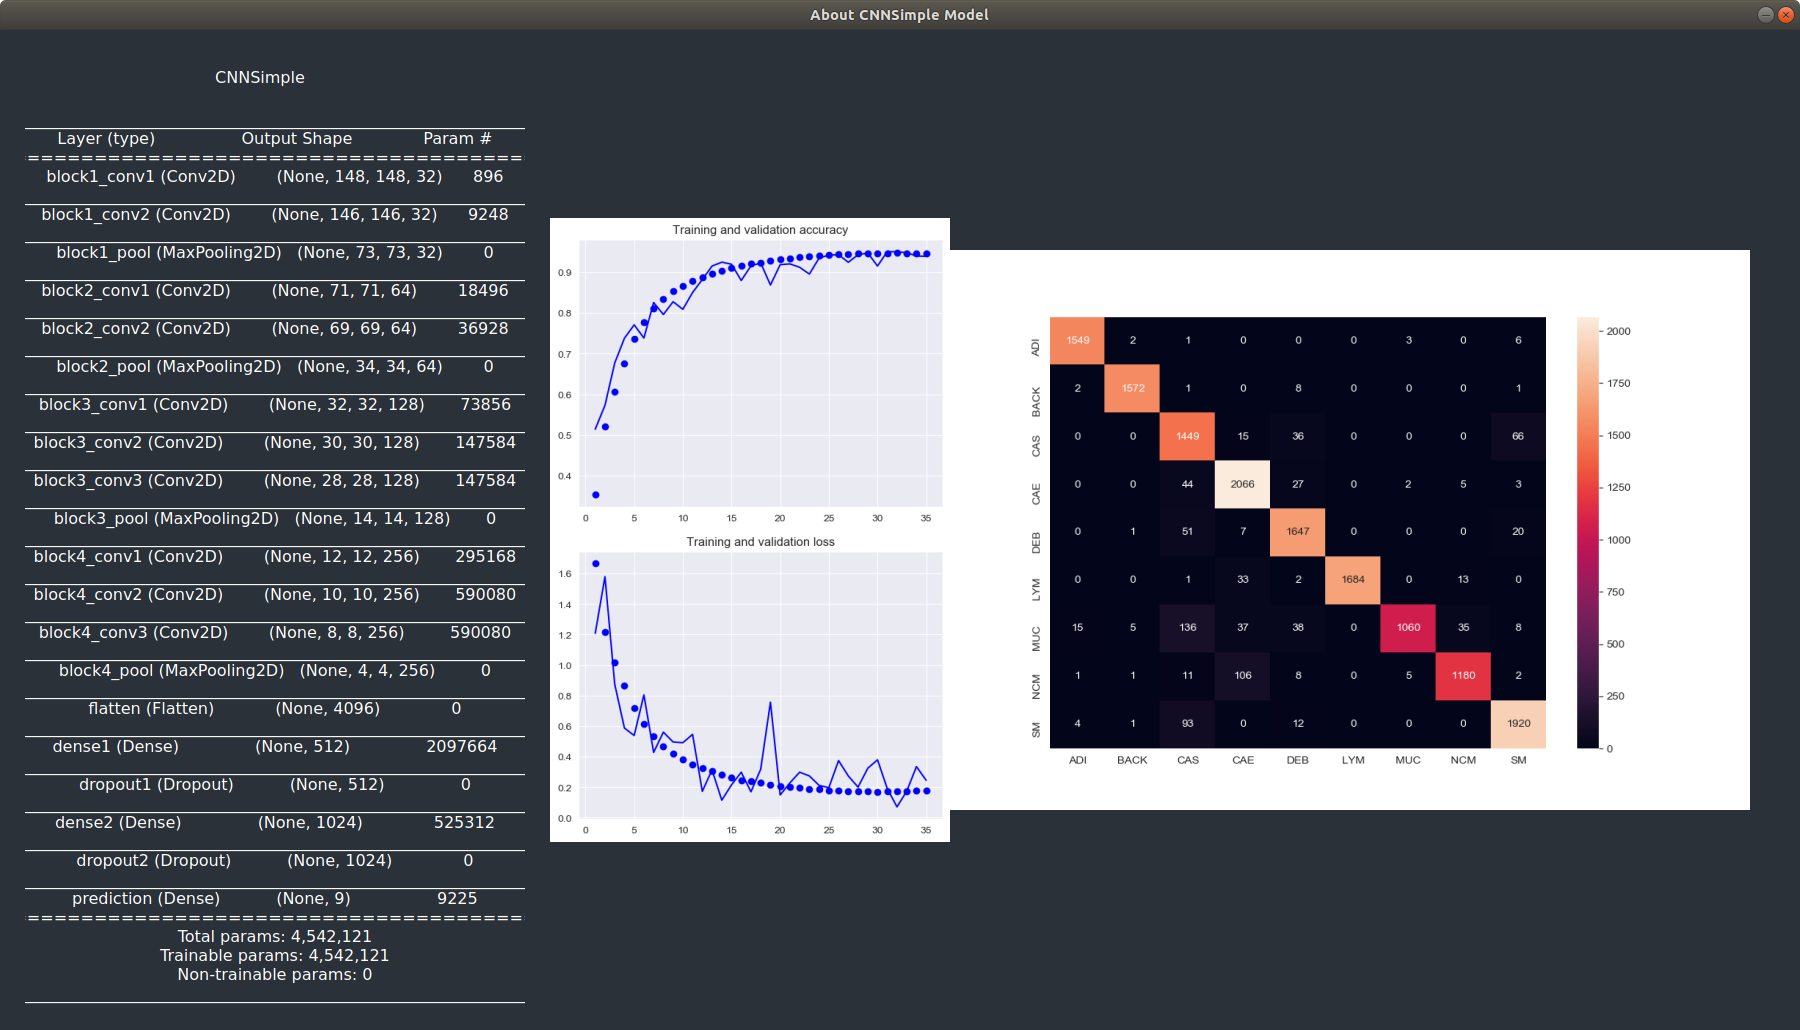
\includegraphics[scale=0.2]{inspect_network.png}
	\caption{CNNSimple Network basic information}
	\label{fig:inspectmodel}
\end{figure}

\section{Basic Use: Predicting Tissue Type}
\label{basicuse}

Main use of the Histopathologic Cancer Detection program is to make it easy and fast to load histopathologic slide and get a prediction on tissue and cancer subtype. In order to load a histopathologic slide, click on \emph{Load\; Image}, and select histopathologic slide for which the prediction is required. Next, select a tissue type of the slide by clicking on \emph{Breast\;Tissue} or \emph{Colorectal\;Tissue} radio button. Afterwards, in order to get tissue and cancer subtype, along with probabilities plot, press \emph{Classify} button (\textcolor{red}{\autoref{fig:predict}}).

\begin{figure}[h]
	\centering
	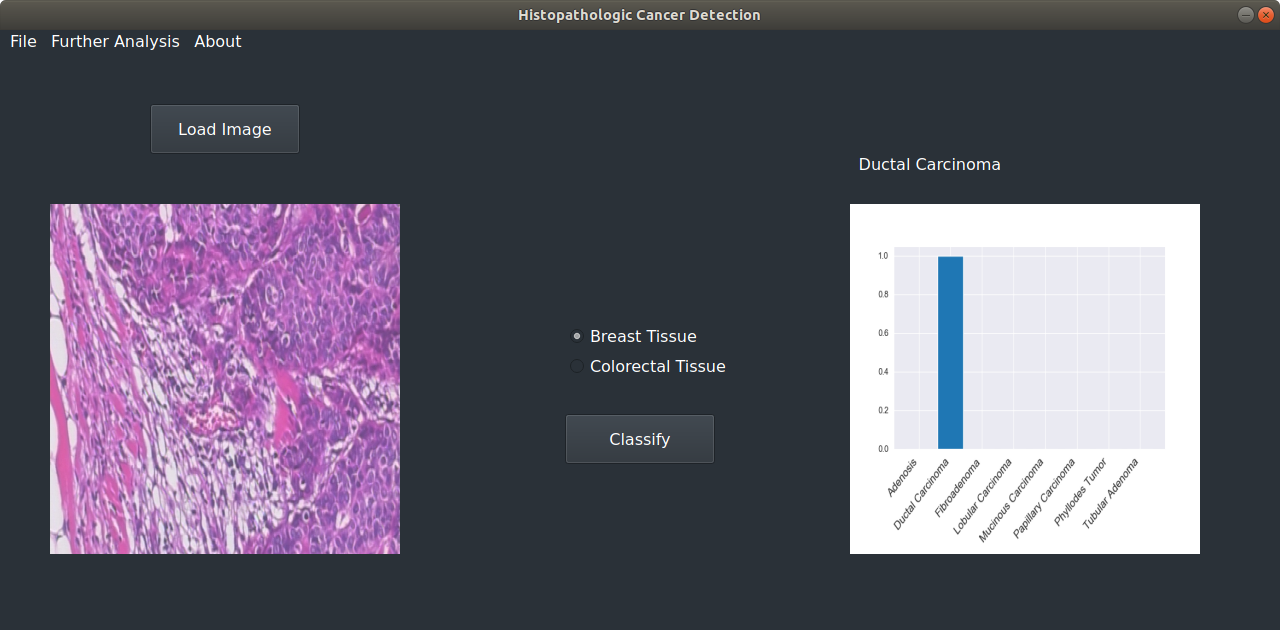
\includegraphics[scale=0.31]{predict.png}
	\caption{Prediction of input histopathologic slide of breast tissue to be ductal carcinoma}
	\label{fig:predict}
\end{figure}

\section{Advanced Use: Visualizing Network Representations}
\label{advuse}

Deep neural networks are highly complex models which have great expressive power and can achieve high accuracy while solving wide range of problems. Unfortunately, with high complexity comes low interpretability, which presents issue, especially in deep learning applications to healthcare. Fortunately, there are several methods to inspect convolutional neural networks, and interpret their output. In this paper, I covered three of them: visualizing heatmaps of class activations, visualizing filters of convolutional layers and visualizing intermediate activations.

\subsection{Visualizing Heatmaps of Class Activations}

Different parts of an image have different weights in networks decision on tissue and cancer subtype classification, and because of that, we can highlight which parts of an image have the highest influence on the networks output. This class of methods is called class activation map visualization, and it produces heatmaps of class activations over input images. A class activation heatmap is a 2D grid of scores associated with a specific output class, computed for every location in any input image, indicating how important each location is with respect to the class under consideration \cite{chollet2018deep}. In order to produce heatmap, go to \emph{Further Analysis $\rightarrow$ Heatmap} (\textcolor{red}{\autoref{fig:heatmap}}).

\begin{figure}[h]
	\centering
	\begin{minipage}{.5\textwidth}
		\centering
		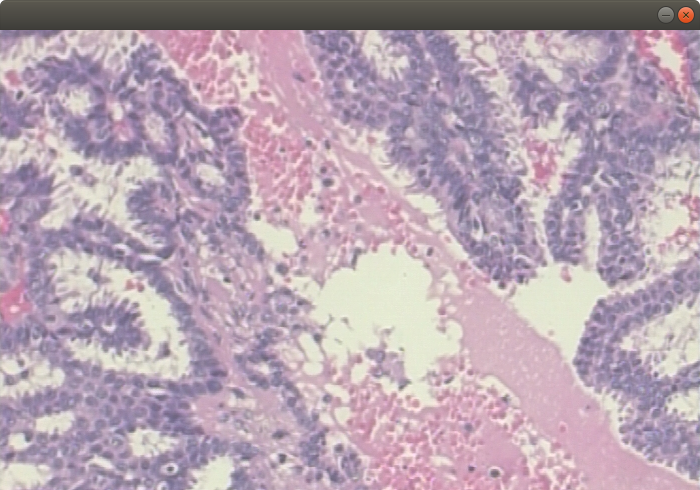
\includegraphics[scale=0.3]{input.png}
		\captionof{figure}{Input image of breast tissue}
		\label{fig:input}
	\end{minipage}%
	\begin{minipage}{.5\textwidth}
		\centering
		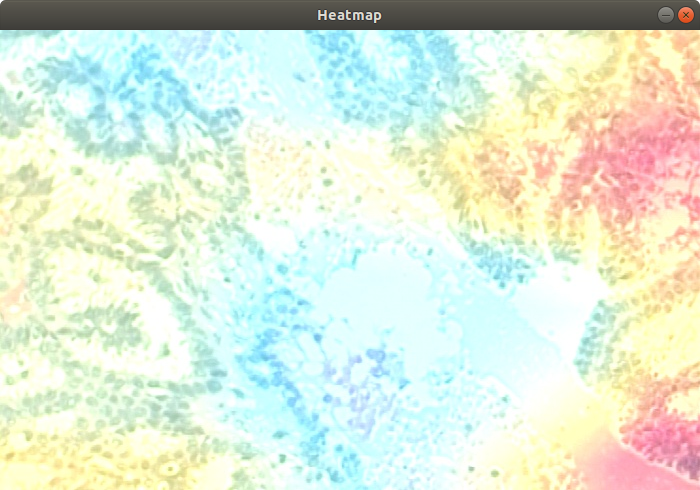
\includegraphics[scale=0.3]{heatmap.png}
		\captionof{figure}{Heatmap of class activations on input image}
		\label{fig:heatmap}
	\end{minipage}
\end{figure}

\subsection{Visualizing Intermediate Activations}

Visualizing intermediate activations consists of displaying the feature maps that are output by various convolutional and pooling layers in a network, given a certain input (the output of a layer is often called its activation, the output of the activation function). This gives a view into how an input is decomposed into the different filters learned by the network \cite{chollet2018deep}. In order to visualize intermediate activations of layers, go to \emph{Further Analysis $\rightarrow$ Class Activations}. Next choose which network layer's intermediate activations should be visualized, along with channel number, or 'all', for visualizing all of layer's channels  (\textcolor{red}{\autoref{fig:interact}}).

\begin{figure}[h]
	\centering
	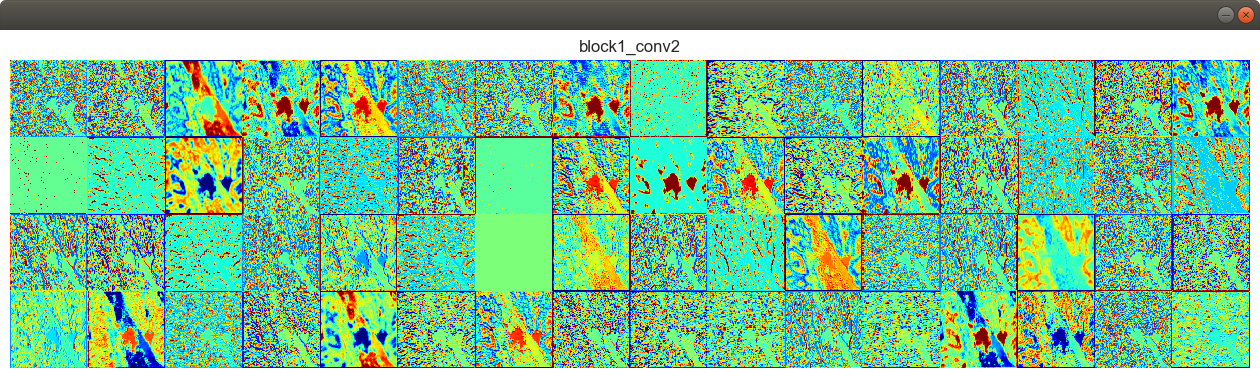
\includegraphics[scale=0.33]{layer_activations.png}
	\caption{Every channel of second convolutional layer of VGG19Simple on a breast tissue input (\textcolor{red}{\autoref{fig:input}}).}
	\label{fig:interact}
\end{figure}

\subsection{Visualizing Filters of Convolutional Layers}

Further analysis is not only dependent on an input image, as we can also inspect feature exractors (filters) of convolutional layers by displaying patterns on which each filter is supposed to respond to. This can be done with gradient ascent in input space: applying gradient descent to the value of the input image of a convnet so as to maximize the response of a specific filter, starting from a blank input image. The resulting input image will be one that the chosen filter is maximally responsive to \cite{chollet2018deep}. In order to visualize filters of convolutional layers, go to \emph{Further Analysis $\rightarrow$ Network Filters}.  Next choose which network convolutional layer's filters should be visualized, along with filter number, or 'all', for visualizing all of layer's filters  (\textcolor{red}{\autoref{fig:filters}}).

\begin{figure}[h]
	\centering
	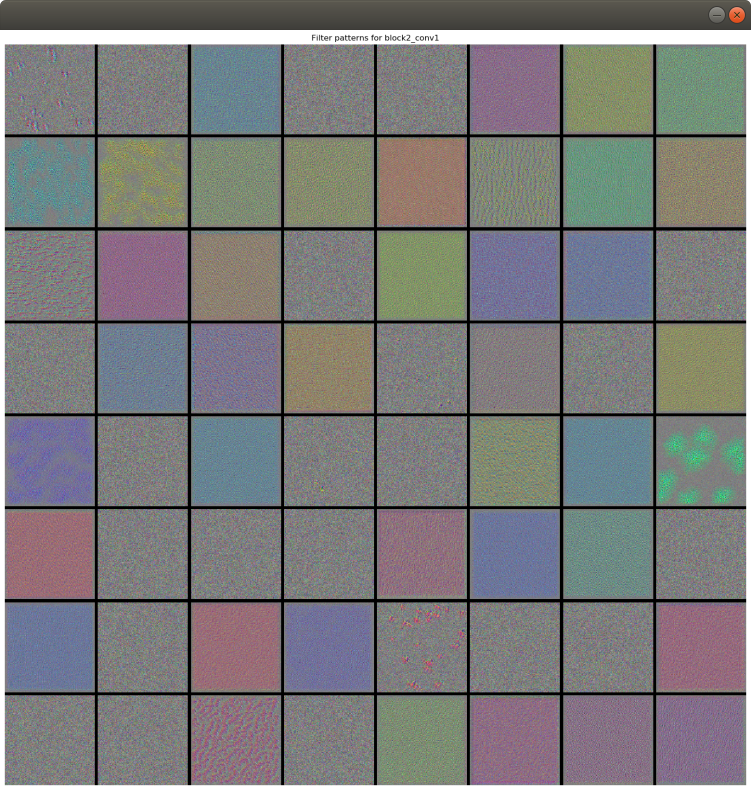
\includegraphics[scale=0.23]{filters.png}
	\caption{Filter patterns for second convolutional layer of CNNSimple network}
	\label{fig:filters}
\end{figure}

\section{Saving Results}
After all predictions have been made, and all further analysis has been conducted, in order to save the results, i.e. save all the images created during the program's execution, go to \emph{File $\rightarrow$ Save}.

\cleardoublepage

\chapter{Developer Documentation} % Developer guide
\label{ch:impl}

Histopathologic Cancer Detection program is divided into four major segments (\textcolor{red}{\autoref{fig:dirdiag}}):
\begin{enumerate}
	\itemsep 0em
	\item Data - includes dataset creation, analysis and visualization
	\item Models - includes creation, training and testing of CNNs
	\item Experiments - includes hyperparameter tuning and network performance assessment and visualization
	\item Graphical User Interface - includes creation of all application windows and their interconnection
\end{enumerate}

\begin{figure}[h]
	\centering
	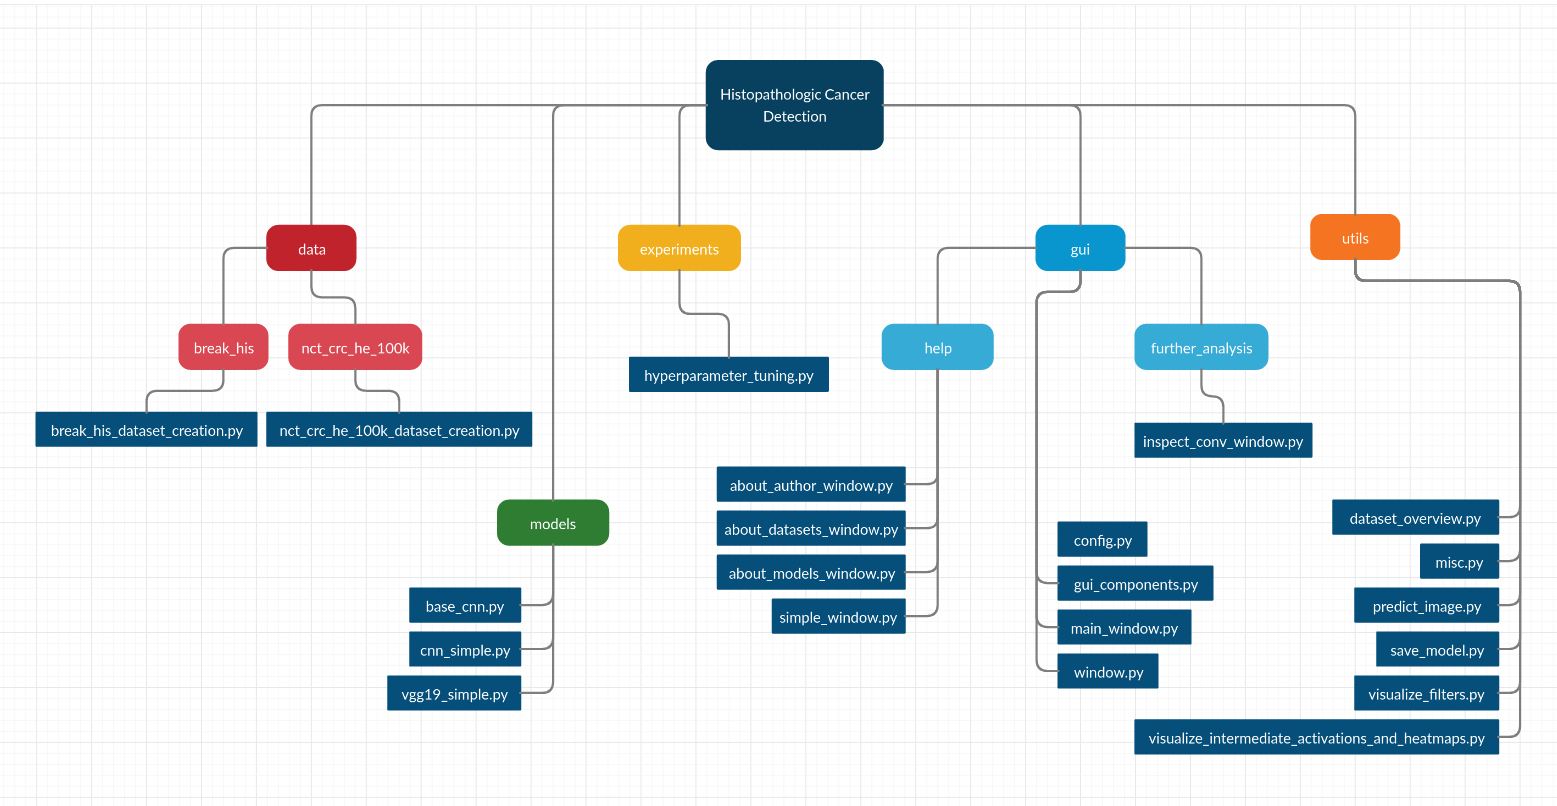
\includegraphics[scale=1.15]{directory_diagram.jpg}
	\caption{Diagram of directories and scripts of Histopathologic Cancer Detection}
	\label{fig:dirdiag}
\end{figure}

\section{Use-Case Diagram}

One of the main goals of the Histopahtologic Cancer Detection program was the ease of use, i.e. straightforward graphical user interface which makes complex operations look quite simple and effortless. Even though there are extremely advanced algorithms with millions of parameters behind the program, GUI was made in such a way that everyone can use it. 

First step is loading the image and selecting tissue type (breast or colorectal tissue), after which classification is being done. At every step of the way, current work can be saved, and new image can be loaded to start the process from scratch. After the classification, it is possible to visualize network representations and perform further analysis of the results by visualizing layer activations, network filters and heatmap (\textcolor{red}{\autoref{fig:usecase}}).

\begin{figure}[h]
	\centering
	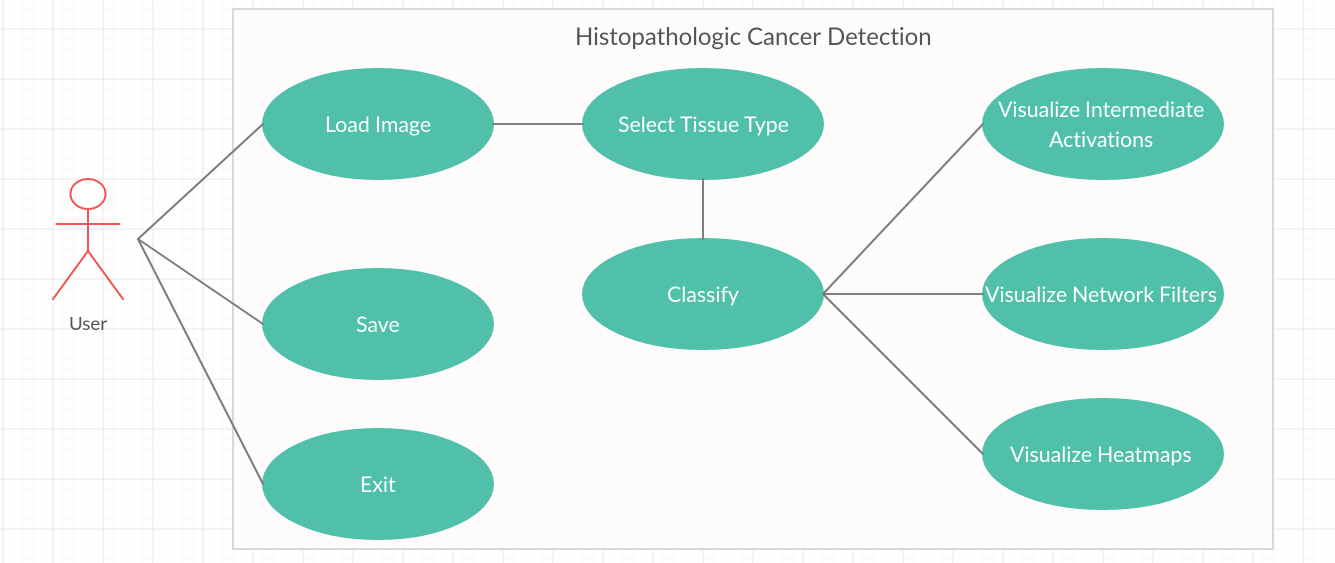
\includegraphics[scale=1]{use_case.jpg}
	\caption{Use-Case Diagram of Histopathologic Cancer Detection}
	\label{fig:usecase}
\end{figure}

\section{Class Diagrams}

Classes of Histopathologic Cancer Detection can be divided into two main components: window classes and neural network classes.

Window class is the base class of all window classes, and it implements common methods, such as setting up window size and central widget. On the other side, MainWindow class is the central point of GUI, as it defines the window which appears when program is run, and every other window is invoked from it (\textcolor{red}{\autoref{fig:class2}}). Window classes, along with their attributed and methods, will be discussed in more detail in Section \textcolor{red}{\ref{gui}}.

\begin{figure}[h]
	\centering
	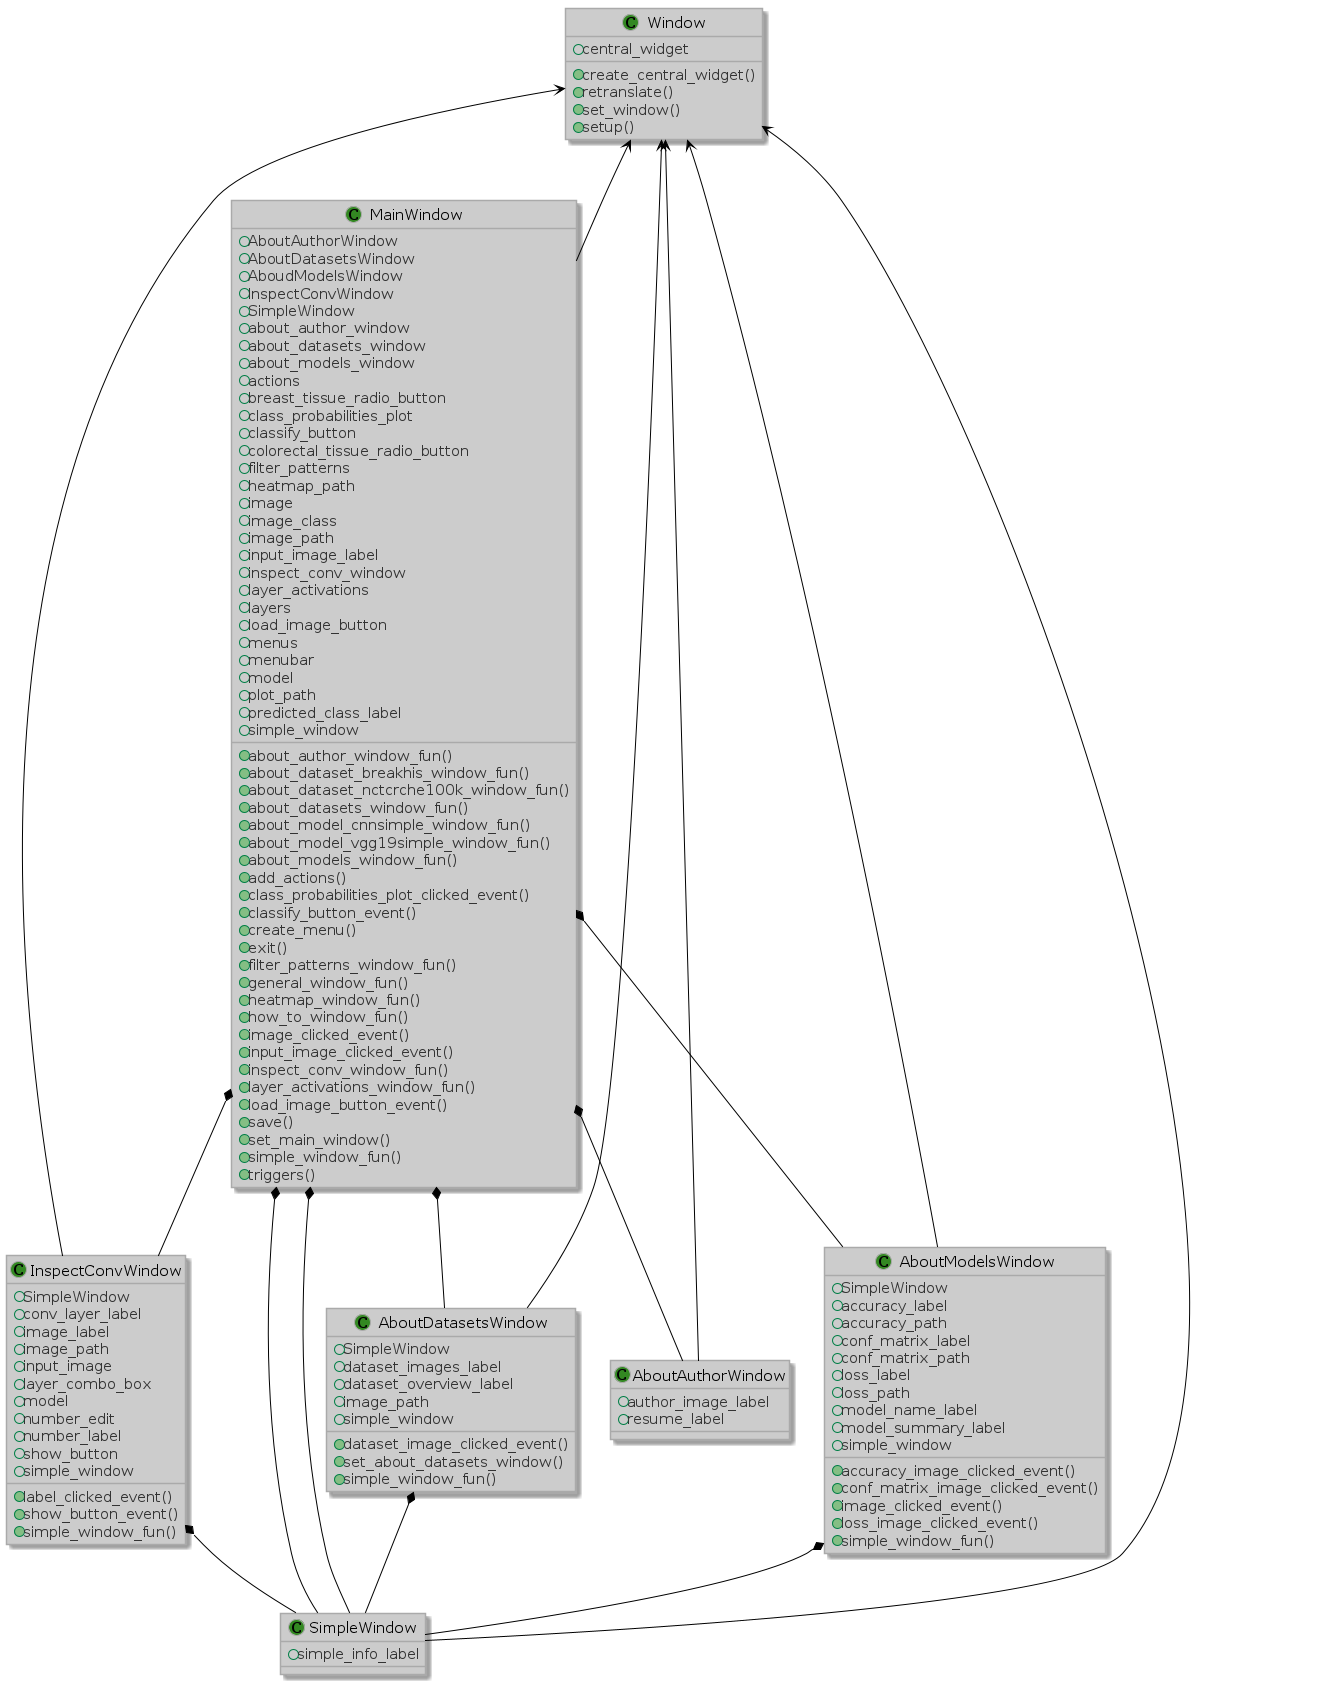
\includegraphics[scale=0.33]{main_class_diagram.png}
	\caption{Class diagram of window classes of Histopathologic Cancer Detection}
	\label{fig:class2}
\end{figure}

\clearpage

BaseCNN class is the common class of all neural network classes, and it contains common attributes, such as dataset name, network name, compile parameters, and common methods, such as creation of data generators, compilation and training of the network. Neural network classes will be discussed in more detail in Section \textcolor{red}{\ref{cnn}}

\begin{figure}[h]
	\centering
	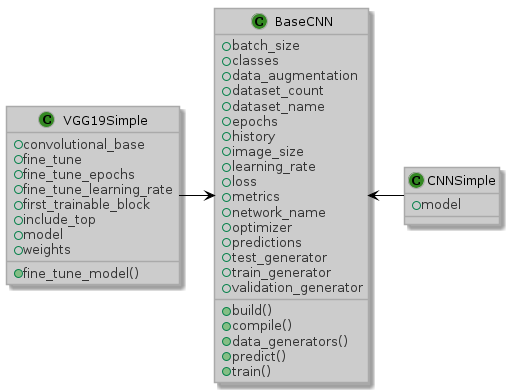
\includegraphics[scale=0.6]{nets_class_diagram.png}
	\caption{Class diagram of neural network classes of Histopathologic Cancer Detection}
	\label{fig:class1}
\end{figure}

\section{Creation of Datasets}

Performance and accuracy of convolutional neural networks relies largely on datasets, i.e. on quality of available data, dataset size, class balance, etc. But before feeding data to the network, if using Keras API, certain dataset structure must be satisfied. More precisely, datasets must have the following structure: train, validation and test directories, each with subdirectory for each class. Scripts responsible for creation of required directory structure are:
\begin{itemize}
	\itemsep 0em
	\item \emph{\textbf{break\_his\_dataset\_creation.py}},
	\item \emph{\textbf{nct\_crc\_he\_100k\_dataset\_creation.py}}.
\end{itemize} 
They work by extracting datasets downloaded from \cite{breakhis_bib}, \cite{nctcrche100k_bib}, creating necessary directory tree and distributing images between created subdirectories. After executing scripts, datasets are ready to be fed into convolutional neural networks (in order to train them), but before that, neural network architecture has to be built.
\clearpage

\section{CNNSimple Implementation}

CNNSimple convolutional neural network (\textcolor{red}{Code \ref{src:py1}}) was created using Keras Sequential model in order to classify images from NCT-CRC-HE-100K dataset, which contains 80.000 images divided into 9 tissue/cancer categories. 

Convolutional base of CNNSimple is composed of four blocks of convolution and max-pooling layers, where first two blocks have two convolution and one max-pooling layer, and last two blocks have three convolution and one max-pooling layer. Each convolution layer has 3x3 convolution window, uses ReLU activation function, and number of feature maps (filters) increases exponentially from 32 to 256. Each max-pooling layer has 2x2 pool size. 

Classification top of CNNSimple is composed of two fully-connected layers, each followed by a dropout layer, and an output (also fully-connected) layer. Fully-connected layers use ReLU activation function, and number of neurons grows from 512 to 1024. Dropout layers use 50\% dropout rate (fraction of neurons which will be ignored in each passing). Output layer uses softmax activation function, and has nine neurons (one neuron per tissue/cancer subtype output). 
\vspace{3mm}
\lstset{caption={CNNSimple network architecture},label=src:py1}
\begin{lstlisting}[language={Python}, basicstyle=\scriptsize]
	model = Sequential()
	model.add(Conv2D(32, (3, 3), activation='relu', input_shape=input_shape,     
	                 name='block1_conv1'))
	model.add(Conv2D(32, (3, 3), activation='relu', name='block1_conv2'))
	model.add(MaxPooling2D((2, 2), name='block1_pool'))
	model.add(Conv2D(64, (3, 3), activation='relu', name='block2_conv1'))
	model.add(Conv2D(64, (3, 3), activation='relu', name='block2_conv2'))
	model.add(MaxPooling2D((2, 2), name='block2_pool'))
	model.add(Conv2D(128, (3, 3), activation='relu', name='block3_conv1'))
	model.add(Conv2D(128, (3, 3), activation='relu', name='block3_conv2'))
	model.add(Conv2D(128, (3, 3), activation='relu', name='block3_conv3'))
	model.add(MaxPooling2D((2, 2), name='block3_pool'))
	model.add(Conv2D(256, (3, 3), activation='relu', name='block4_conv1'))
	model.add(Conv2D(256, (3, 3), activation='relu', name='block4_conv2'))
	model.add(Conv2D(256, (3, 3), activation='relu', name='block4_conv3'))
	model.add(MaxPooling2D((2, 2), name='block4_pool'))
	model.add(Flatten(name='flatten'))
	model.add(Dense(512, activation='relu', name='dense1'))
	model.add(Dropout(0.5, name='dropout1'))
	model.add(Dense(1024, activation='relu', name='dense2'))
	model.add(Dropout(0.5, name='dropout2'))
	model.add(Dense(9, activation='softmax', name='prediction'))
\end{lstlisting} 

\section{Transfer Learning}

Although CNNs are a powerful tool for image classification, in order to achieve high accuracy, large amount of data is needed. Problem occurs when only small dataset is available (as is often in healthcare, ex. BreakHis dataset). In such cases transfer learning can be used: take model trained on large dataset and transfer knowledge to small dataset, i.e. freeze convolutional base, and only train classification top of the network. Main idea is that early layers of convolutional base learns low-level features applicable across all images, such as edges and patterns.

\subsection{VGG19Simple Implementation}

VGG19Simple convolutional neural network (\textcolor{red}{Code \ref{src:py2}}) was created using Keras Graphical API in order to classify images from BreakHis dataset, which contains 2.000 images divided into 8 tissue/cancer categories. 

Convolutional base of VGG19Simple is VGG19 pre-built network pre-trained on ImageNet dataset (without top classification part), using imagenet weights.

Classification top of CNNSimple is composed of two fully-connected layers, each followed by a dropout layer, and an output (also fully-connected) layer. Fully-connected layers use ReLU activation function, and number of neurons grows from 512 to 1024. Dropout layers use 50\% dropout rate (fraction of neurons which will be ignored in each passing). Output layer uses softmax activation function, and has nine neurons (one neuron per tissue/cancer subtype output). 

\vspace{3mm}
\lstset{caption={VGG19Simple network architecture},label=src:py2}
\begin{lstlisting}[language={Python}, basicstyle=\scriptsize]
	input = Input((150, 150, 3))
	convolutional_base = VGG19(weights='imagenet', include_top=False,
	                           input_tensor=input)
	for layer in convolutional_base.layers:
		layer.trainable = False
	x = Flatten(name='flatten')(convolutional_base.output)
	x = Dense(512, activation='relu', name='dense_1')(x)
	x = Dropout(0.5, name='dropout_1')(x)
	x = Dense(1024, activation='relu', name='dense_2')(x)
	x = Dropout(0.5, name='dropout_2')(x)
	x = Dense(8, activation='softmax', name='predictions')(x)
	
	model = Model(input, x)
\end{lstlisting} 

\section{Experiments and Results}

Performance of neural networks is determined by how well will it generalize, i.e. how high accuracy will it achieve on previously unseen data (if it performs well on training data, but underachieves on test data, it is said that CNN overfits). In order to prevent overfitting, number of techniques can be used: increase size of dataset, change network architecture or apply hyperparameter tuning techniques, which consist of selecting a set optimal hyperparameters for learning algorithm. Selection of such parameters for networks is done in \textbf{\emph{hyperparameter\_tuning.py}}. First step consists of defining hyperparameter dictionary with parameters and values to be tested, such as number of epochs for which network is to be trained, optimization techniques, etc. Next step consists of training network with all combination of parameters and values defined, after which network performances are compared in order to determine the best hyperparameter set.

CNNSimple network trained on NCT-CRC-HE-100K dataset was trained for 50 epochs, using RMSProp optimizer with learning rate of 0.00002, using categorical crossentropy loss function. Before feeding data to the network, data augmentation (applying random transformations in order to produce more images, such as translation, rotation, sheer) has been used. In order to judge performance of the network, accuracy metrics function was employed. CNNSimple achieved 91.3\% validation and 91.3\% test accuracy, and 0.18 validation and 0.28 test loss (\textcolor{red}{\autoref{fig:cnnperf}}).

\begin{figure}[h]
	\centering
	\subfigure[\scriptsize Accuracy]{\label{fig:a}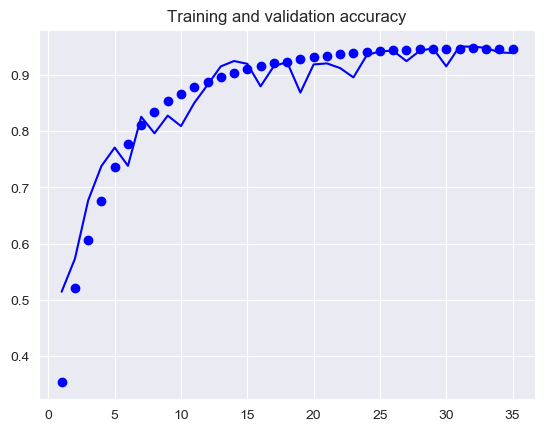
\includegraphics[width=65mm]{cnn_acc.png}}
	\subfigure[\scriptsize Loss]{\label{fig:b}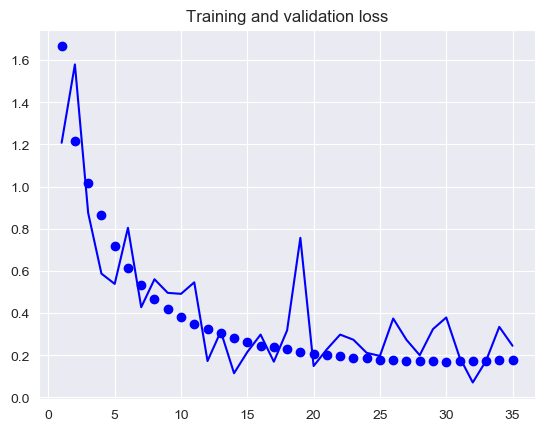
\includegraphics[width=65mm]{cnn_loss.png}}
	\caption{CNNSimple performance on NCT-CRC-HE-100K train and validation dataset}
	\label{fig:cnnperf}
\end{figure}

\clearpage
VGG19Simple network trained on BreakHis dataset was trained for 150 epochs, using Adam optimizer with learning rate of 0.0001, using categorical crossentropy loss function. Before feeding data to the network, data augmentation (applying random transformations in order to produce more images, such as translation, rotation, sheer) has been used. In order to judge performance of the network, accuracy metrics function was employed. After training network with frozen convolutional base, last convolutional block was unfreezed, and network was trained again using Adam optimizer with learning rate of 0.00005. VGG19Simple achieved 61.7\% validation and 62.1\% test accuracy, and 1.18 validation and 0.62 test loss (\textcolor{red}{\autoref{fig:vgg19perf}}).

\begin{figure}[h]
	\centering
	\subfigure[\scriptsize Accuracy]{\label{fig:vgg19perf}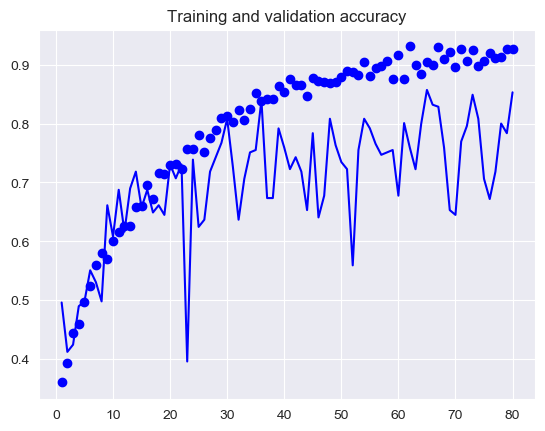
\includegraphics[width=65mm]{vgg19_acc.png}}
	\subfigure[\scriptsize Loss]{\label{fig:b}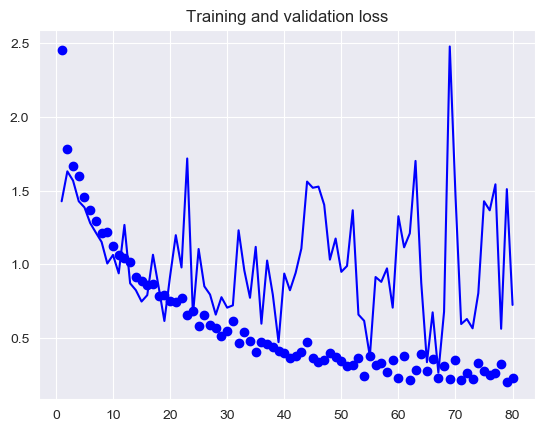
\includegraphics[width=65mm]{vgg19_loss.png}}
	\caption{VGG19Simple performance on BreakHis train and validation dataset}
	\label{fig:vgg19perf}
\end{figure}

Another way of interpreting network performance is by plotting confusion matrix, which is a summary table of correct and incorrect predictions broken down by each class (\textcolor{red}{\autoref{fig:cnncf}, \autoref{fig:vgg19cf}}).

\begin{figure}[h]
	\centering
	\begin{minipage}{.5\textwidth}
		\centering
		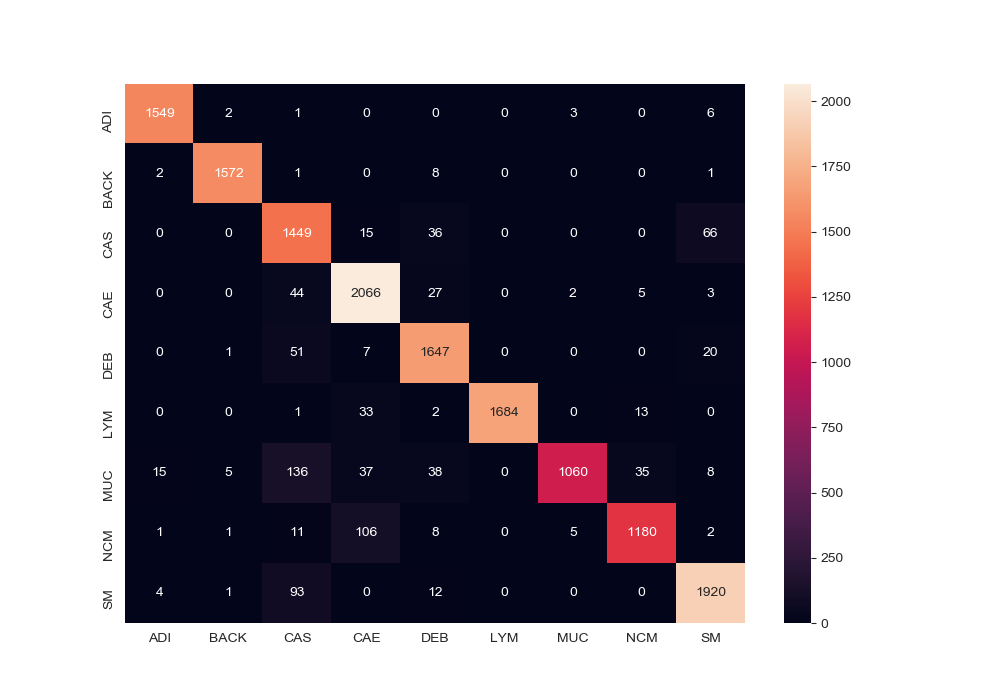
\includegraphics[scale=0.31]{cnn_cf.png}
		\captionof{figure}{Confusion Matrix of CNNSimple on NCT-CRC-HE-1OOK test dataset}
		\label{fig:cnncf}
	\end{minipage}%
	\begin{minipage}{.5\textwidth}
		\centering
		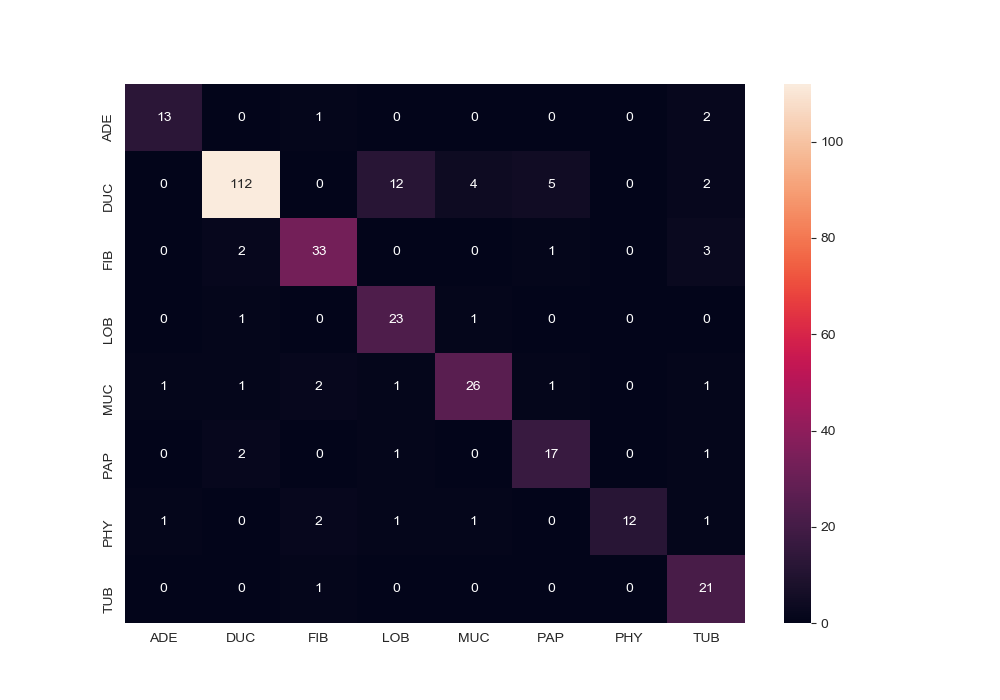
\includegraphics[scale=0.31]{vgg19_cf.png}
		\captionof{figure}{Confusion Matrix of VGG19Simple on BreakHis test dataset}
		\label{fig:vgg19cf}
	\end{minipage}
\end{figure}

\clearpage

\section{Graphical User Interface} \label{gui}

In order to make using program simple and straightforward, graphical user interface using PyQt5 has been created. Following window classes have been constructed:
\begin{itemize}
	\itemsep 0em
	\item Window class in \textbf{\emph{window.py}}, used as base class for every other window, which contains primitive functions for setting up window, creating central widget, etc.
	\item AboutAuthorWindow class in \textbf{\emph{about\_author\_window.py}}, which contains two labels (containing image and CV respectively)
	\item AboutDatasetsWindow class in \textbf{\emph{about\_datasets\_window.py}}, which contains two labels (containing dataset sample images and dataset overview numbers respectively)
	\item AboutModelsWindow class in \textbf{\emph{about\_models\_window.py}}, which contains five labels (containing network name, network architecture, accuracy, loss and confusion matrix plots respectively)
	\item SimpleWindow class in \textbf{\emph{simple\_window.py}}, which contains one image label
	\item InspectConvWindow class in \textbf{\emph{inspect\_conv\_window.py}}, which contains three labels (containing convolution layer text, number text and image respectively), button (with associated action), combo box (containing network layer names)  and line edit (for input of numbers)
	\item MainWindow class in \textbf{\emph{main\_window.py}}, which connects every other window and provides main program functionality 
\end{itemize}
In addition, every window specific information is located in \textbf{\emph{config.py}}, such as window sizes, positions and names of labels, paths to images, etc. GUI component definitions are located in \textbf{\emph{gui\_components.py}}.

\subsection{Main Window}

MainWindow class is the central part of the GUI, as it defines the window which pops up when program is started. It has menu bar from which every other window can be reached, and central widget which contains input image, tissue-type radio buttons, classify button and output class label and probabilities plot. Function \emph{classifyButtonEvent}, associated with \emph{classifyButton} is the integral part of the class, as it loads network based on the input image tissue type, classifies it, and writes output to labels.


\section{Utilities}

For program to work seamlessly, certain utilities needed to be implemented:
\begin{itemize}
	\itemsep 0em
	\item \textbf{\emph{dataset\_overview.py}}, used for obtaining basic information about dataset, such as sample images and image distribution per class
	\item \textbf{\emph{misc.py}}, containing function for reading file contents 
	\item \textbf{\emph{predict\_image.py}}, used for predicting class to which an image belongs
	\item \textbf{\emph{save\_model.py}}, used for saving neural network information and performance after being trained, such as arguments, architecture, accuracy, loss and confusion matrix plots, filters, etc.  
	\item \textbf{\emph{visualize\_filters.py}}, used for visualizing network filter patterns
	\item \textbf{\emph{visualize\_intermediate\_activations\_and\_heatmaps.py}}, used for visualizing intermediate activations of network and heatmaps of class activation
\end{itemize}

\section{Implementing Additional Features}

In addition to the ease of use of Histopathologic Cancer Detection program, source code was written in such a way to make expanding scope (problem space) of the program by including additional features quite simple and fast. If new tissue type (ex. lung tissue), along with tissue/cancer subtype classification was to be added to the program, it would be accomplished in four steps:
\begin{enumerate}
	\itemsep 0em
	\item \textbf{Creating dataset} \\
	Obtaining dataset of new tissue type, and preparing dataset to be fed to Keras-built CNN, which includes creating appropriate directory structure
	\item \textbf{Building CNN} \\
	Crating new convolutional neural network class inherited from BaseCNN by defining data generator transformations, network architecture, etc.
	\item \textbf{Fine-tuning CNN} \\
	Defining hyperparameter dictionary and training neural networks in order to increase classification accuracy and prevent overfitting
	\item \textbf{Extending GUI} \\
	Adding additional radio button to MainWindow class, and extending action associated with classify button, as well as further analysis actions, to use newly created network
\end{enumerate}
\cleardoublepage

\chapter{Conclusion}
\label{ch:sum}

Over the past decade convolutional neural networks have achieved results few expected would be possible in such a short time period, and recently they have been successfully implemented in healthcare industry \cite{miotto2018deep}. Histopathological Cancer Detection program shows that deep learning algorithms can be applied in the field of histopathology, and achieve high performance results in order to reduce workload from doctors, and help speed up the process. More importantly, it overcomes one of the major drawbacks of deep learning algorithms, which is the notion of algorithms being 'black-boxes', i.e. not being highly interpretable. By implementing multiple techniques to further analyze network and its decisions, it is possible to explain and clarify network outputs and determine whether such reasoning is correct or not.

\section{Future Work}

After completing the thesis and creating program for histopathologic cancer detection on breast and colorectal tissue, there are multiple ways of extending the scope of the program: adding more tissue types in order to increase solving power, adding additional ways to further analyze results, and improving graphical user interface in order to make it even more straightforward to use.

ACDC@LUNGHP\footnote{Automatic Cancer Detection and Classification in Whole-slide Lung Histopathology 2019} challenge provides dataset for lung cancer histopathologic detection, which could be used for extending the program scope. DigestPath2019\footnote{Digestive-System Pathological Detection and Segmentation Challenge 2019} challenge provides dataset for colorectal histopathologic cancer detection, which could be used to improve accuracy of already existing CNNSimple network. Additional histopathology datasets are publicly available, such as ECDP2020 grand challenge dataset and ANHIR\footnote{ Automatic Non-rigid Histological Image Registration} challenge dataset.

Another way to visually interpret and further analyze CNN classification results and increase interpretability of the networks is by using deconvolutional neural networks (DCNNs) \cite{zeiler2011adaptive}.
\cleardoublepage

% Appendices
\appendix
\chapter{Convolutional Neural Networks}
\label{appx:simulation}

Convolutional Neural Networks for image classification \cite{krizhevsky2012imagenet} take image as an input, process it, and output category to which that image belongs. Processing part consists of a series of layers through which image is propagated in order to learn features, which in turn determine to which class an image belongs. (\textcolor{red}{\autoref{fig:cnn1}}).

\begin{figure}[h]
	\centering
	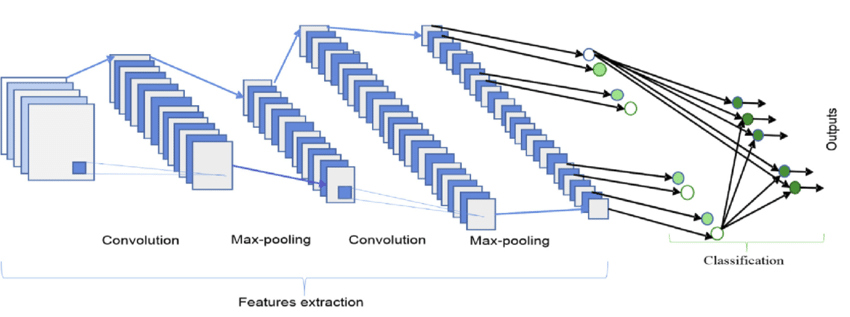
\includegraphics[scale=0.5]{cnn.png}
	\caption{Convolutional Neural Network consisting of two Convolutional layers, two Max-Pooling layers, Flatten layer and two Fully-Connected (Dense) layers}
	\label{fig:cnn1}
\end{figure}

Most commonly used layers in CNN architectures are convolutional layer, max-pooling layer, flatten layer, dense layer and dropout layer.

\section{Convolutional Layer}

Convolutional layer is the building block of the CNN architecture. Its primary purpose is to extract features from input image, such as edges, lines, curves, colors. As we go deeper inside the network, it starts identifying more complex features, such as shapes, objects. This layer consists of multiple filters (feature extractors, usually 3$\times$3 matrices) whose parameters need to be learned.
\section{Max-Pooling Layer}

Max-Pooling layer is located after a series of convolutional layers in CNN architecture. It is a downsampling method which reduces dimensionality, thus decreasing number of parameters and computational power needed in order to train the network, while retaining important features and patterns. It is achieved by applying a max filter to non-overlapping subregions (usually 2$\times$2 matrices), thus reducing the size of each feature map by a factor of 2.

\section{Flatten Layer}

Output of the convolutional base of the network (series of convolutional and max-pooling layers) is a two-dimensional matrix, and before feeding that data to the classification top of the network, it needs to be transformed. Flatten layer reshapes the output matrix to a vector, thus removing all dimensions but one in the process, making the data prepared for the series of fully-connected layers.

\section{Fully-Connected Layer}

After the high-level features of the image have been detected, series of fully-connected (dense) layers is attached to the top of the network in order to classify image into a label. Dense layers consist of huge number of nodes (neurons), which provide a way of learning non-linear combinations of features outputted by convolutional base, and determine which features most correlate to a particular class.

\section{Dropout Layer}

Fully-Connected layer contains the most parameters in the network, and as a result neurons develop co-dependency amongst each other during training, which leads to overfitting the data (not generalizing well on new, unseen images). In order to prevent that, dropout layers are positioned right after dense layers in CNN architecture as a means of regularizing the network. Dropout consists of randomly ignoring (dropping out) fraction of neurons of fully-connected layer, which in turn makes network learn more robust features, and achieve better performance.
\clearpage

\cleardoublepage

% Bibliography (mandatory)
\addcontentsline{toc}{chapter}{\biblabel}
\printbibliography[title=\biblabel]
\cleardoublepage

\end{document}
